
\section{Simulated data - the testing paradise}
\label{mmf-sec:simulated data}
Just like in \autoref{ch:variantcalling}, the novelty of the approach leads to the issue of no gold standard dataset, with which to evaluate the performance of a new method. While there are low coverage WGS datasets of cancer patients, none of them have validated signatures associated with them. So again simulated data is the optimal starting point to allow both optimisation of parameters as well as granular detection of artefacts which can originate from any step starting from sequencing over mapping to the signature deconvolution. 

\subsection{Sequencing errors - there is always a cleaner data}
\label{mmf-sec:cleanSim}
To judge the ability of our approach to filter out sequencing errors, we first simulated ``clean`` sequencing reads with neither germline or somatic variants with the ART simulation suite \cite{Huang2011}. As current estimates of Illumina sequencing is in the range of 1 in 666 to 1 in 1149 \cite{Stoler2021} which is significantly higher than even the highest tumour mutational burdens of  cancers (melanoma: 1 in 5k; tobacco smoking lung cancer: 1 in 100k) it is very important to be able to eliminate as much of the  background noise of sequencing errors as possible.

\begin{figure}[!ht]
\centering
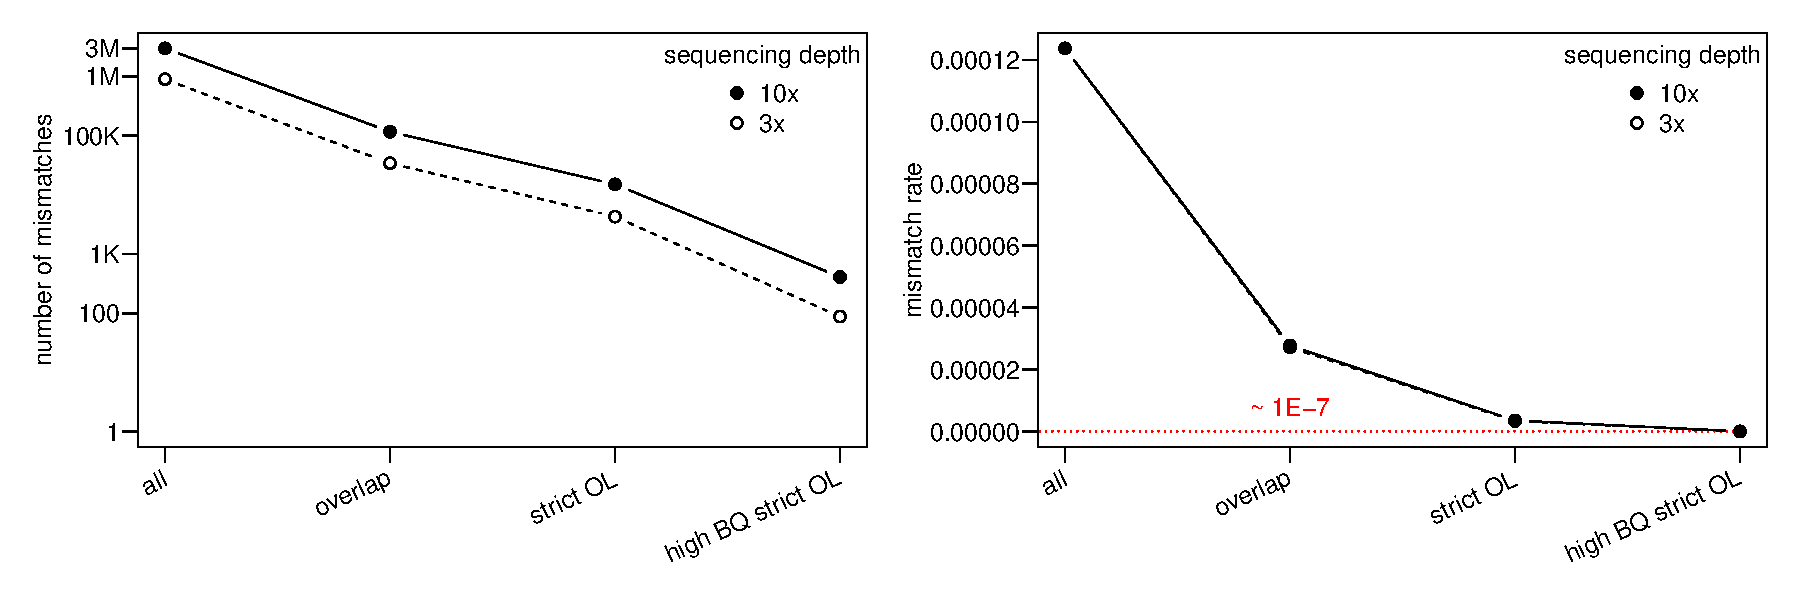
\includegraphics[width=.99\linewidth]{Figures/mismatchrateCleanSequencing.pdf}
\caption[Mismatchrate of different filtering methods]{Mismatchrate of different filtering methods on sequencing data simulated with ART\cite{Huang2011} for both 10x and 3x coverage; Mismatches correspond to simulated sequencing errors; all: no filters, overlap: only use the overlapping parts of paired end reads with consensus building (\protect\autoref{mmf-sec:consensus}), strict OL: overlap but reads \emph{must} agree, high BQ strict OL: strict OL with high BQ in both variants; A) Absolute counts B) counts from A normalised by the number of analysed bases all: all aligned bases, other: number of bases in read overlap}\label{fig:mmf-mismatchrate}
\end{figure}

By only using high base quality mismatches, where both reads agree on the mismatch 99.98\% of all sequencing errors can be eliminated and only 1 in 10M bases will be wrongly counted as a variant (\autoref{fig:mmf-mismatchrate}). This false discovery rate is multiple orders of magnitude lower than before and in a similar range to normal mutationally driven cancers tumour mutational burden \cite{Alexandrov2020,Lawrence2013a}.

\todo[inline]{show data with germline filtering}